\documentclass[10pt]{beamer}

%STANDARD PREAMBLE
%https://tex.stackexchange.com/questions/68821/is-it-possible-to-create-a-latex-preamble-header
\usepackage{/Users/miw267/Repos/latex_preamble/beamer_preamble}
%\usepackage{/Users/miw267/Repos/csci246_spring2025/slides/preambles/beamer_preamble_for_CSCI246}


%%%
% SPECIFIC TO THIS DOCUMENT 
%%%
\let\warning\relax
\usepackage{fourier} % has warning  and danger symbols. However, it makes the bottoms tuff bold. 

\renewcommand{\ELBO}{\texttt{ELBO}}
\renewcommand{\Q}{\mathcal{Q}}


%%%%
% DOCUMENT 
%%%
\title{04/02/2026: Classic Score Matching}
\author{Reference: Hyv\"arinen, A. (2005). \textit{Estimation of non-normalized statistical models by score matching.} }
\date{CSCI 546: Diffusion Models}

\begin{document}
\maketitle

%\begin{frame}{Table of contents}
%  \setbeamertemplate{section in toc}[sections numbered]
%  \tableofcontents[hideallsubsections]
%\end{frame}

\begin{frame}{Table of contents}
  \setbeamertemplate{section in toc}[sections numbered]
  \setbeamertemplate{subsection in toc}[subsections numbered]
  \tableofcontents
\end{frame}





\section{Course Logistics}



\begin{frame}{Final Project Notes}
\begin{myredbox}[title=Announcement]

I've provided specs about the final project in the syllabus.
\end{myredbox}
\end{frame}


\begin{frame}{Reading Survey}

\begin{enumerate}
	\item Describe score matching.  For example, how does it work and when would you use it?
\end{enumerate}
	
\end{frame}




\section{Mini-Lecture: Diffusion}


\begin{frame}[standout]
Mini-Lecture: Diffusion \\
See previous slide deck
\end{frame}




\section{Group Work}



\begin{frame}[standout]
Group Work\\
See previous slide deck
\end{frame}







\section{Mini-Lecture: Score Matching}

\begin{frame}{A fundamental problem}

Let $\+X \in \R^d$ be a random vector.
\pause
\vfill 
Any set of non-negative functions $\set{q_\+\theta(\+x)}_{\+\theta \in \Theta}$ parameterized by $\+\theta$ can be used to construct $\set{p_\+\theta(\+x)}_{\+\theta \in \Theta}$, a family of probability densities over $\+X$.
\pause
\vfill 
Since probability density functions \textbf{must} integrate to 1, we set
\[ p_\+\theta(\+x) = \frac{q_\+\theta(\+x)}{Z_\+\theta},\] 
where $Z_\+\theta := \int q_\+\theta(\+x) d\+x$ is a normalizing constant.
\pause
\vfill 
\colorbox{red!30}{\textbf{The problem.}} What if we can't compute $Z_\+\theta$?
\pause 
\vfill 
\colorbox{green!30}{\textbf{A solution.}} We show how to train and sample from these models using \alert{score matching}, which matches the \textbf{score functions} of the model to the data.
\end{frame}

\begin{frame}{Score function}

\colorbox{green!30}{\textbf{Definition.}} The \textbf{score function} (or \textit{Stein score}) is the gradient of the log likelihood with respect to the data vector $\+x$:

\[\+s(\+x) = \nabla_\+x \ln p_\+\theta(\+x) \]

\vfill 
\begin{figure} 
\includegraphics[width=.3\textwidth]{images/score_function} 
\caption{ Illustration of score function for a mixture of two-dimensional Gaussians.}
\end{figure}

\only<2-3>{
\vfill 
\colorbox{yellow!30}{\textbf{Poll.}} Interpretation? 
} \only<3>{The score function is a vector field pointing to the direction of \alert{steepest increase} in the log likelihood.
} 
\vspace{-.3cm}
\only<4-5>{
\vfill 
\colorbox{yellow!30}{\textbf{Poll.}} Why is this useful?}\only<5>{ \; We don't need the normalizing constant! \[\nabla_\+x \ln p_\+\theta(\+x) = \nabla_\+x \ln q_\+\theta(\+x) - \red{\cancel{\nabla_\+x \ln Z_\+\theta}} = \nabla_\+x \ln q_\+\theta(\+x). \]
} 

\end{frame}



\begin{frame}{Langevin Sampling}

\colorbox{yellow!30}{\textbf{Poll.}} How can we use the score function to obtain a sample $\+x$ from the probability distribution with density $p$? 

\vspace{-.2cm}

\vfill 
\begin{figure} 
\includegraphics[width=.3\textwidth]{images/score_function} 
\end{figure}
\vspace{-.3cm}
\pause 
\vfill 
\colorbox{purple!30}{\textbf{Solution.}} Start with an initial value $\+x^^0$, and then iterate the following Markov chain steps:
\[\+x^^t = \+x^^{t-1} + \eta  \; \labeledgreenmathbox{score function}{\nabla_\+x \ln p_\+\theta(\+x)}  + \sqrt{2 \eta} \+\epsilon^^t, \qquad t=1,2, \hdots T.\]
\hfill where $\+\epsilon^^t \sim \N(\+0, \+I)$ and $\eta$ is a learning rate.
\pause 
\vfill 
\colorbox{red!30}{\textbf{Theorem.}} As $T \to \infty$, $\+x^^T$ becomes an independent sample from $p_\+\theta(\+x).$
\end{frame}

\begin{frame}{Langevin Sampling}

\textbf{Langevin Sampling.} Start with an initial value $\+x^^0$, and then iterate the following Markov chain steps:
\[\boxed{\+x^^t = \+x^^{t-1} + \eta  \; \nabla_\+x \ln p_\+\theta(\+x)  + \sqrt{2 \eta} \+\epsilon^^t, \qquad t=1,2, \hdots T.}\]
%where $\+\epsilon^^t \sim \N(\+0, \+I)$ and $\eta$ is a learning rate.

\only<2>{
\vfill 
\begin{figure} 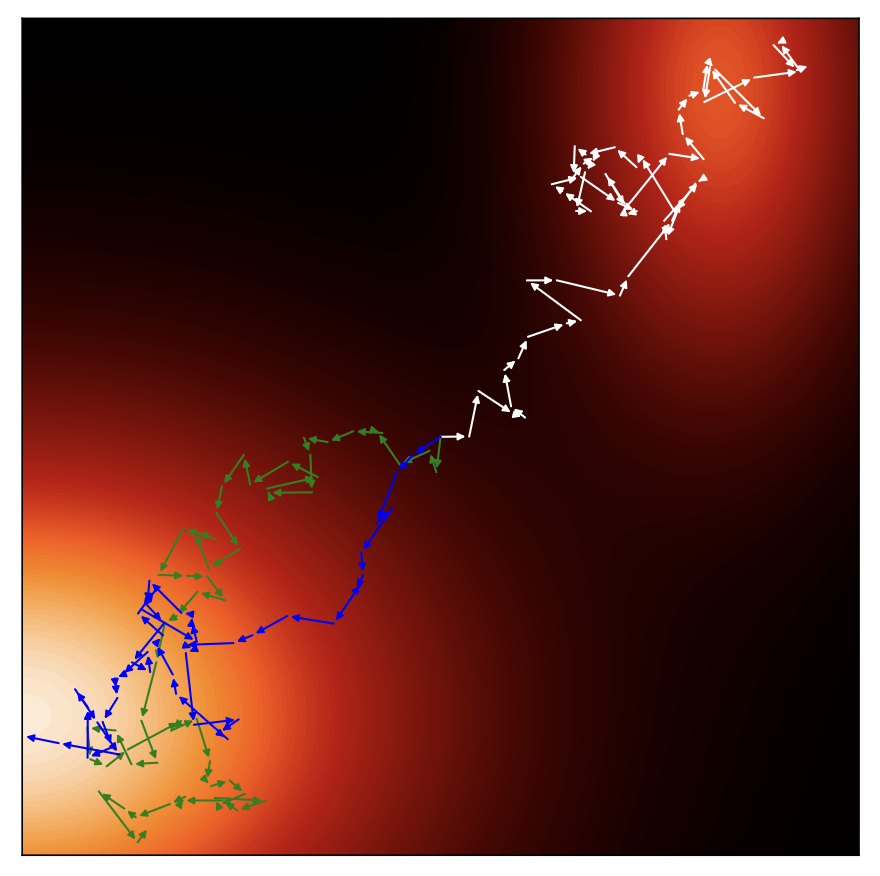
\includegraphics[width=.45\textwidth]{images/langevin_sampling} 
\caption{Three trajectories, all starting from the center of the plot.}
\end{figure}
\vspace{-.3cm}
}

\only<3->{
\vfill 
\begin{figure} 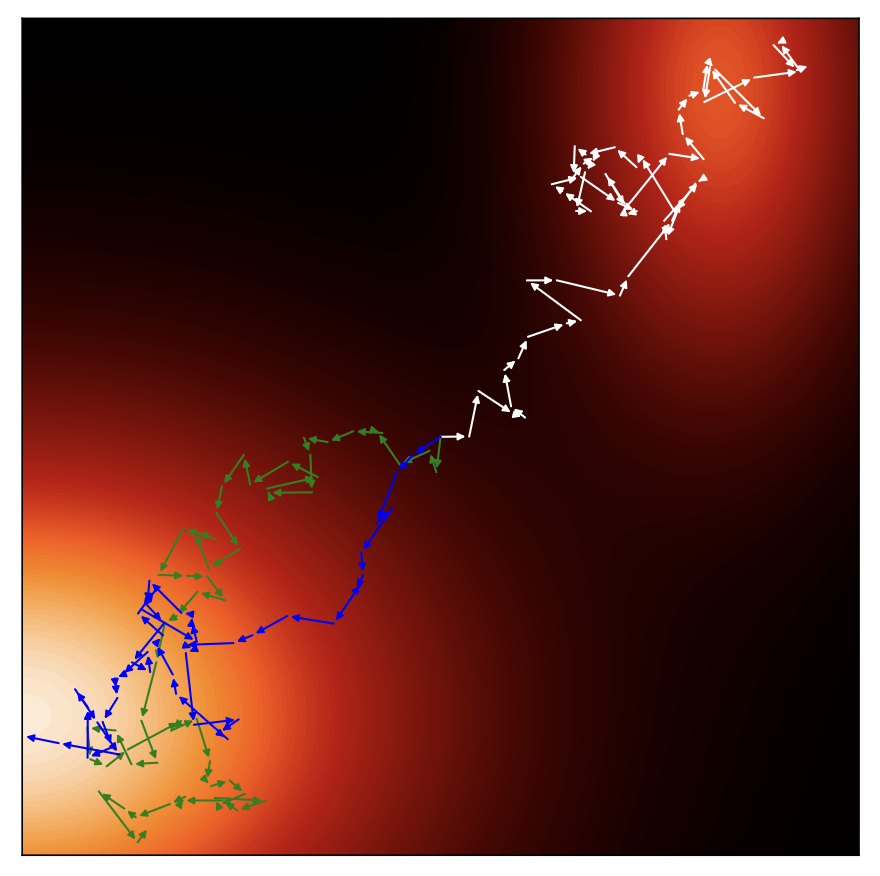
\includegraphics[width=.3\textwidth]{images/langevin_sampling} 
\caption{Three trajectories, all starting from the center of the plot.}
\end{figure}
\vspace{-.4cm}
}


\only<3-4>{
\colorbox{yellow!30}{\textbf{Poll.}} Why is this useful?  
}

\only<4>{
\colorbox{green!30}{\textbf{Solution.}} We don't need the probability distribution to be normalized!
} 
\only<5->{
\colorbox{red!30}{\textbf{Problem.}} But how do we \alert{learn} $\nabla_\+x  \ln p_\+\theta(\+x)$ from data?  
}

\only<6>{
\colorbox{green!30}{\textbf{Solution.}} \texttt{Score matching} to the rescue!
} 
\end{frame}

\begin{frame}{Score Matching}

\only<1>{
Let 
\begin{itemize}
	\item $ p_0(\+x)$ be the density of the true data generating distribution
	\item $ p_\+\theta(\+x)$ be the density of our model.
\end{itemize}
}

\only<2->{
Then the \textbf{score matching} training loss is given by
\[ J(\+\theta) = \int \half \; || \labeledgreenmathbox{model score}{\nabla_\+x  \ln p_\+\theta(\+x)} -  \labeledredmathbox{true score}{\nabla_\+x  \ln p_0(\+x)}||^2 \;  p_0(\+x) \, d\+x\]
}

\only<3-4>{
\colorbox{yellow!30}{\textbf{Poll.}} What is the interpretation of this training loss?  
}

\only<4>{
\colorbox{purple!30}{\textbf{Solution.}} It's the expected squared error between the model score and the true score. (Multiplied by a half).
} 


\only<5->{
\vfill 
\colorbox{purple!30}{\textbf{Idea.}} If we want to learn a modeled score function in a flexible manner, we could train a neural network $s(\+x,\+\theta)=\nabla_\+x  \ln p_\+\theta(\+x)$ within this loss function. 
}


\only<5-6>{
\colorbox{purple!30}{\textbf{Problem.}} There's a \red{blocker} to doing this. What is it?
} \only<6>{Even if we have collected a bunch of observations $\+x_1, \+x_2, \hdots \+x_n$, there's no way to know the \red{true score} of these observations!} 


	
\end{frame}



\begin{frame}{Hyv\"arinen's Solution}

\only<1->{
\colorbox{purple!30}{\textbf{Problem.}} We want to train a neural network $s(\+x,\+\theta)$ via the loss function
\[ J(\+\theta) = \int \half \; || \labeledgreenmathbox{model score}{s(\+x,\+\theta)} -  \labeledredmathbox{true score}{\nabla_\+x  \ln p_0(\+x)}||^2 \;  p_0(\+x) \, d\+x,\]
but we don't know the \red{true score}.
}

\only<2->{
\vfill 
\colorbox{purple!30}{\textbf{Solution.}} Using integration by parts, we can rewrite this as 
\[ J(\+\theta) = \int \; \bigg\{ \nabla \cdot \greenmathbox{s(\+x,\+\theta)} + \half   || \greenmathbox{s(\+x,\+\theta)}||^2 \; \bigg\} \; p_0(\+x) \, d\+x,\]
where $\nabla \cdot s = \sum_{i=1}^d \frac{\partial s_i}{\partial x_i} $ is the divergence operator.
}

\only<3-4>{
\vfill
\colorbox{purple!30}{\textbf{Implication.}} Who cares?
} \only<4>{Now the integrand doesn't refer to the \red{true score} at all!}

\only<5-6>{
\vfill
\colorbox{purple!30}{\textbf{Implementation.}} But we also don't know $p_0(\+x)$. So how to use in practice?
} \only<6>{If we have $N$ observations from $p_0(\+x)$, then we can use a Monte Carlo approximation:

\[  J(\+\theta) \approx \frac{1}{N} \; \sum_{i=1}^N \bigg\{ \nabla \cdot \greenmathbox{s(\+x_i,\+\theta)} + \half   || \greenmathbox{s(\+x_i,\+\theta)}||^2 \; \bigg\}  \] 
}

\end{frame}

\section{Lightning Chat}

\begin{frame}[standout]
\href{https://molkars.github.io/csci546-mocabee-shaffer-spring2026/score-matching/}{\alert{\underline{Lightning Chat}}}
\end{frame}






\end{document}

